\documentclass{beamer}

\usepackage[utf8]{inputenc}
\usepackage{hyperref}

\usetheme{Berkeley}
\beamertemplatenavigationsymbolsempty
\setbeamertemplate{headline}{}
 
\title{Clustering in FoodChain-Lab}
\date{}
 
\begin{document}
\maketitle

\section{Tasks}
\begin{frame}
	\begin{itemize}
		\item Perform a clustering base the following workflow: \url{https://github.com/SiLeBAT/BfROpenLabResources/raw/master/GitHubPages/workflows/FCL_Example.zip}
		\item Cluster all French primary producers based on their city.
		\item That means all stations from the same city should be put into one meta-station.
	\end{itemize}
\end{frame}
 
\section{1}
\begin{frame}
	\begin{center}
  		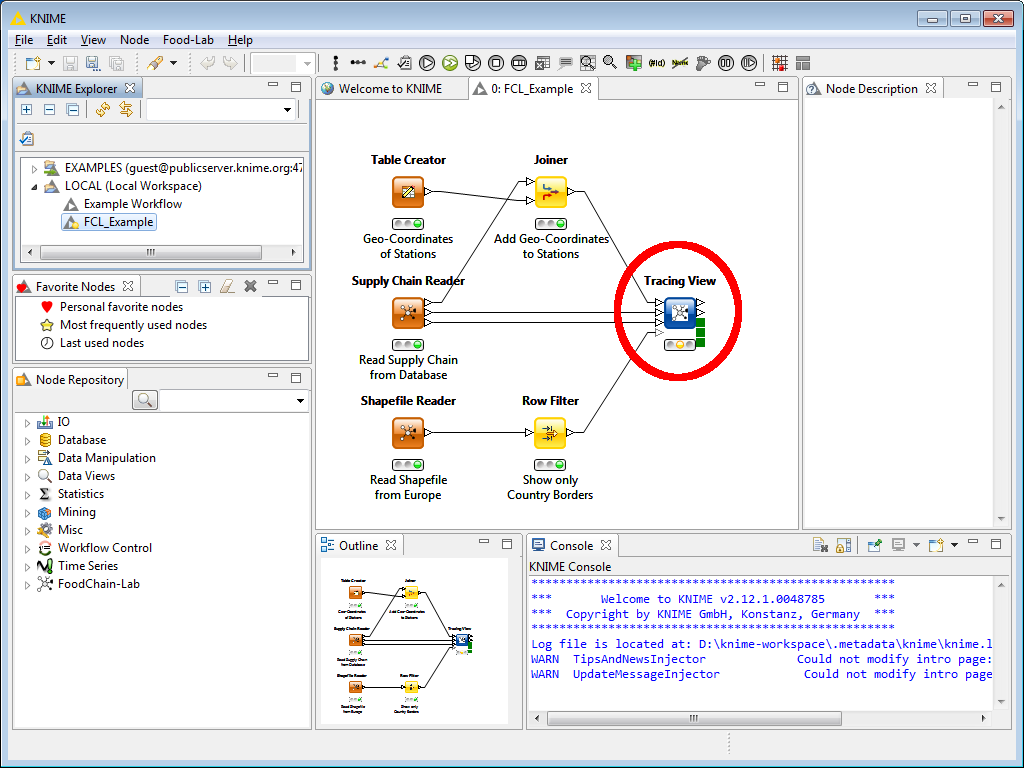
\includegraphics[height=0.6\textheight]{1.png}
	\end{center}
	\begin{itemize}
		\item Import the Example Workflow from \url{https://github.com/SiLeBAT/BfROpenLabResources/raw/master/GitHubPages/workflows/FCL_Example.zip}.
		\item Open the \textbf{Tracing View} by double-clicking on it.
	\end{itemize}
\end{frame}

\section{2}
\begin{frame}
	\begin{center}
  		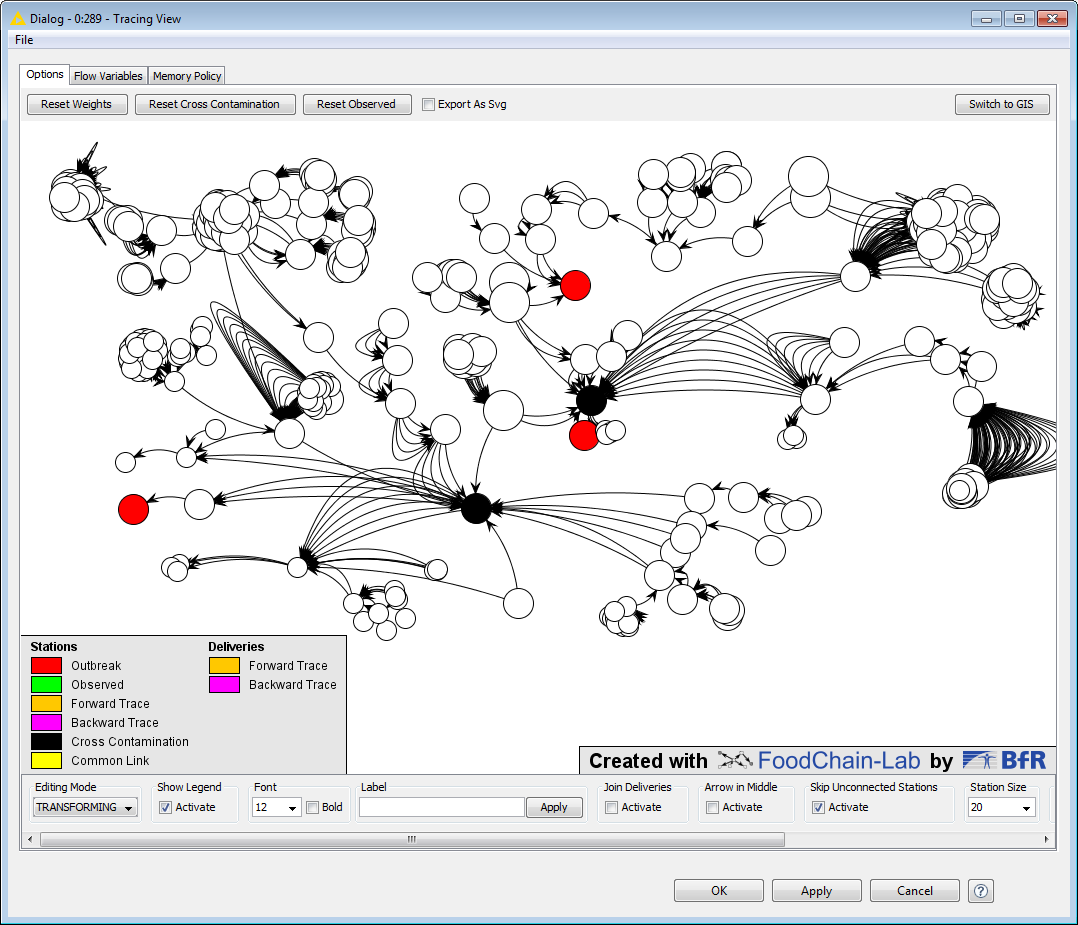
\includegraphics[height=0.6\textheight]{2.png}
	\end{center}
	\begin{itemize}
		\item A window showing the delivery network should open now.
	\end{itemize}
\end{frame}

\section{3}
\begin{frame}
	\begin{center}
  		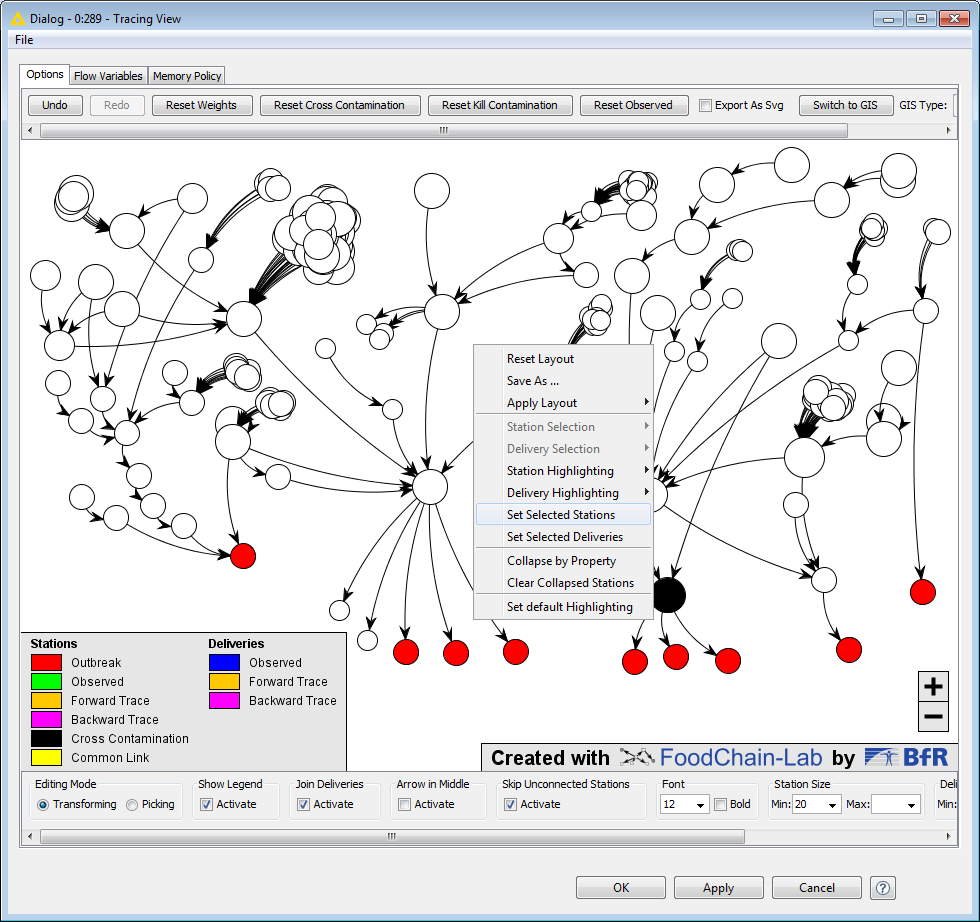
\includegraphics[height=0.6\textheight]{3.png}
	\end{center}
	\begin{itemize}
		\item Right click in the graph to open the context menu and select \textbf{Set Selected Stations}.
	\end{itemize}
\end{frame}

\section{4}
\begin{frame}
	\begin{center}
  		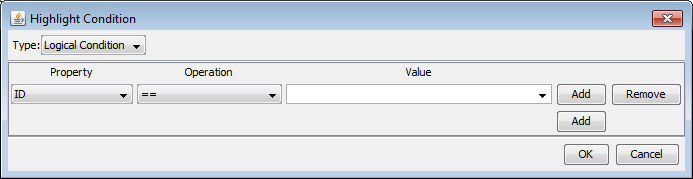
\includegraphics[width=0.9\textwidth]{4.png}
	\end{center}
	\begin{itemize}
		\item You should see this dialog now.
		\item Press the button in the red circle to change the \textbf{Property} value.
	\end{itemize}
\end{frame}

\section{5}
\begin{frame}
	\begin{center}
  		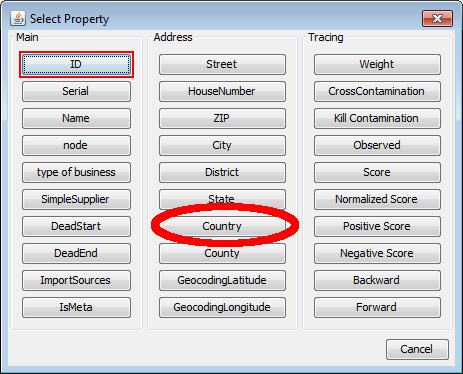
\includegraphics[width=0.7\textwidth]{5.png}
	\end{center}
	\begin{itemize}
		\item Select "Country".
	\end{itemize}
\end{frame}

\section{6}
\begin{frame}
	\begin{center}
  		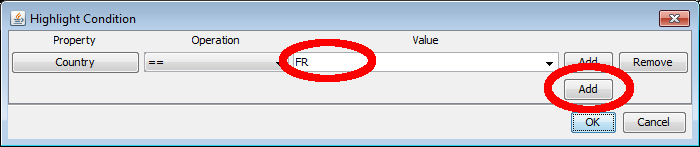
\includegraphics[width=0.9\textwidth]{6.png}
	\end{center}
	\begin{itemize}
		\item Now select "FR" as \textbf{Value}, since we want to cluster stations in France.
		\item Afterwards press \textbf{Add} to add another condition.
	\end{itemize}
\end{frame}

\section{7}
\begin{frame}
	\begin{center}
  		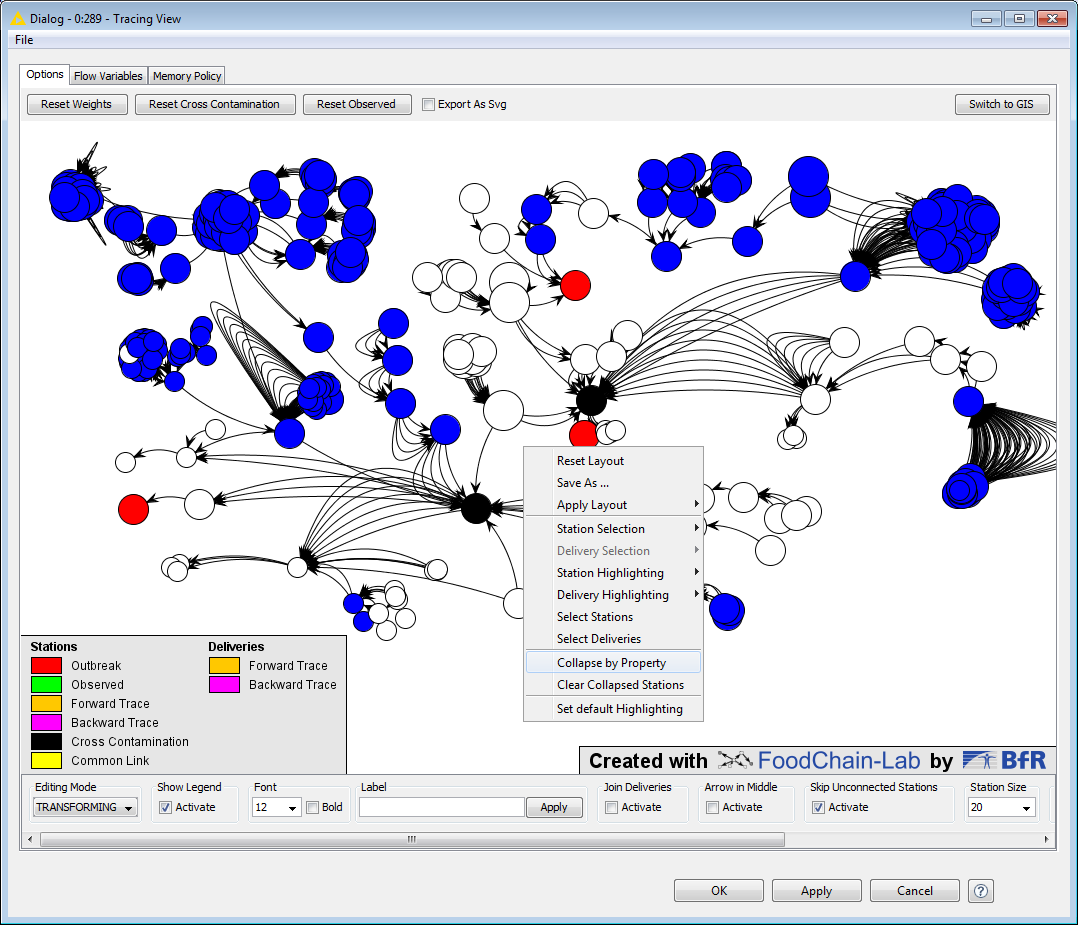
\includegraphics[width=0.9\textwidth]{7.png}
	\end{center}
	\begin{itemize}
		\item For the new condition select "type of business" as \textbf{Property} and "Primary Producer" as \textbf{Value}, since we want to cluster primary producers only.
		\item Now press \textbf{OK}.
	\end{itemize}
\end{frame}


\section{8}
\begin{frame}
	\begin{center}
  		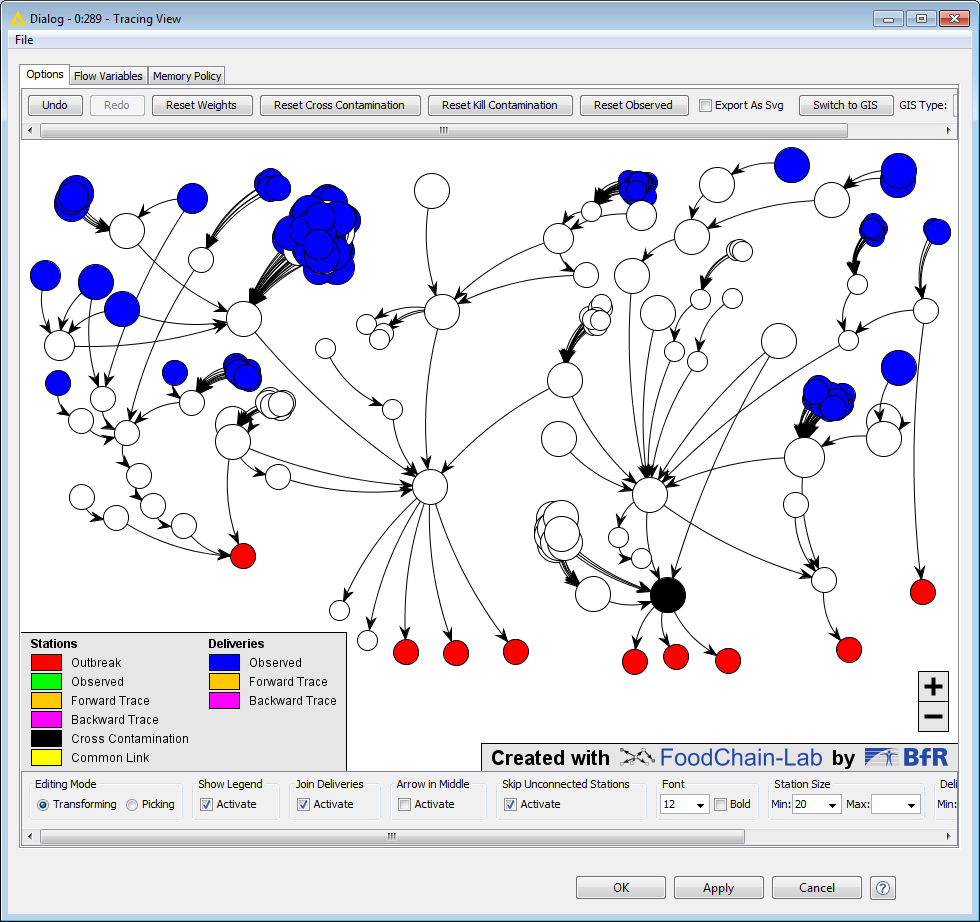
\includegraphics[height=0.6\textheight]{8.png}
	\end{center}
	\begin{itemize}
		\item All French primary producers are seleted now, which is indicated by the blue color.
	\end{itemize}
\end{frame}

\section{9}
\begin{frame}
	\begin{center}
  		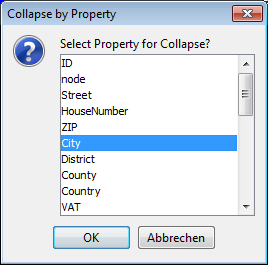
\includegraphics[height=0.6\textheight]{9.png}
	\end{center}
	\begin{itemize}
		\item Right click in the graph to open the context menu and select \textbf{Collapse by Property} to cluster the selected stations.
	\end{itemize}
\end{frame}

\section{10}
\begin{frame}
	\begin{center}
  		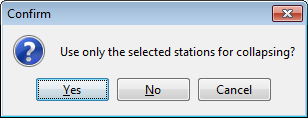
\includegraphics[width=0.7\textwidth]{10.png}
	\end{center}
	\begin{itemize}
		\item Select \textbf{Yes} to only cluster selected stations.
	\end{itemize}
\end{frame}

\section{11}
\begin{frame}
	\begin{center}
  		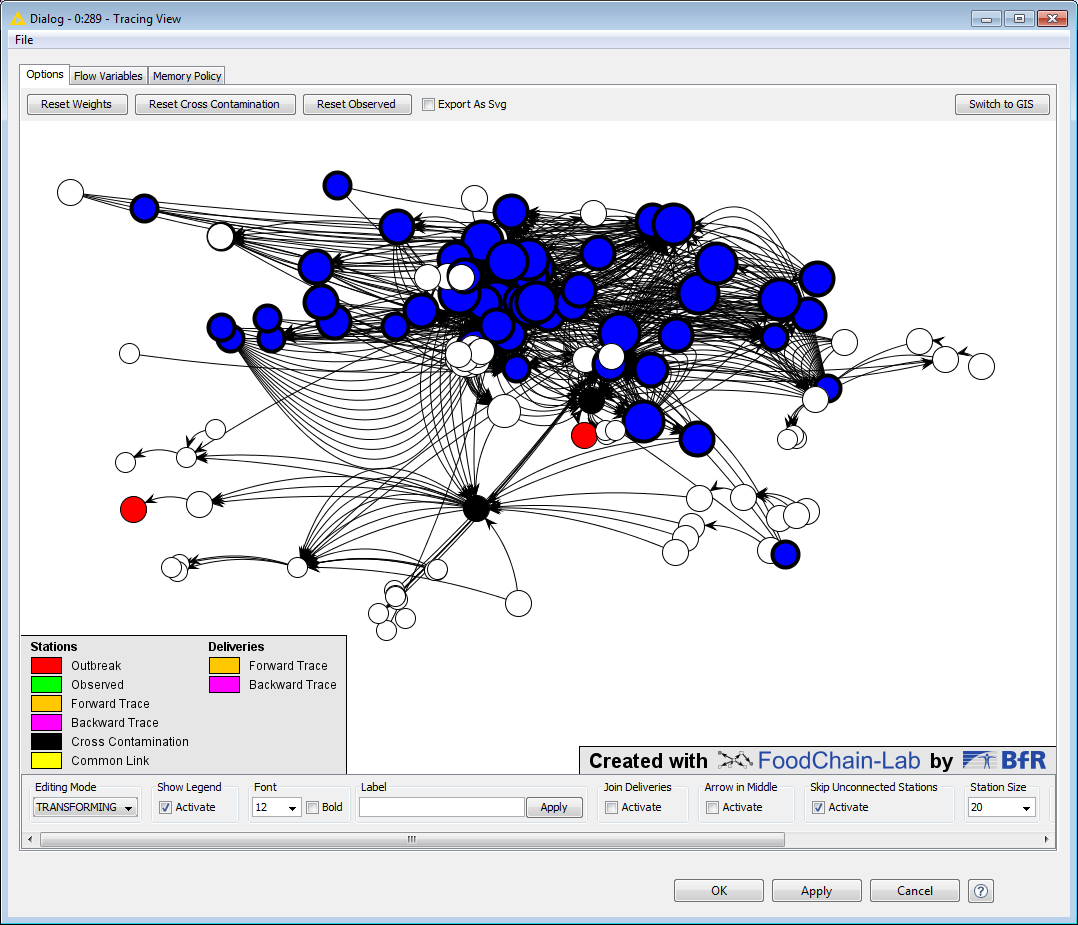
\includegraphics[height=0.5\textheight]{11.png}
	\end{center}
	\begin{itemize}
		\item The clustering will be done on city level. That means all stations from the same city will be merged.
		\item Select \textbf{City} and press \textbf{OK}.
	\end{itemize}
\end{frame}

\section{12}
\begin{frame}
	\begin{center}
  		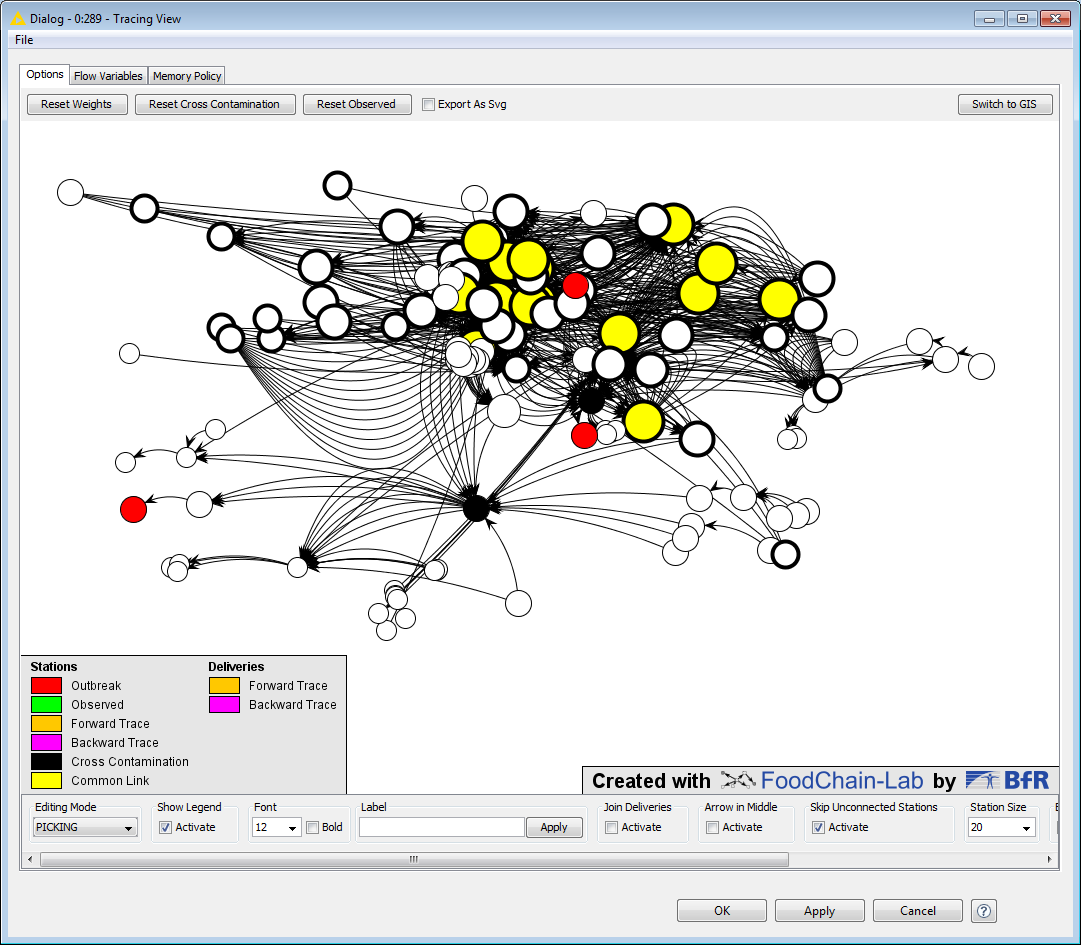
\includegraphics[height=0.5\textheight]{12.png}
	\end{center}
	\begin{itemize}
		\item Just press \textbf{OK}, since we do not want to exclude any cities.
	\end{itemize}
\end{frame}

\section{13}
\begin{frame}
	\begin{center}
  		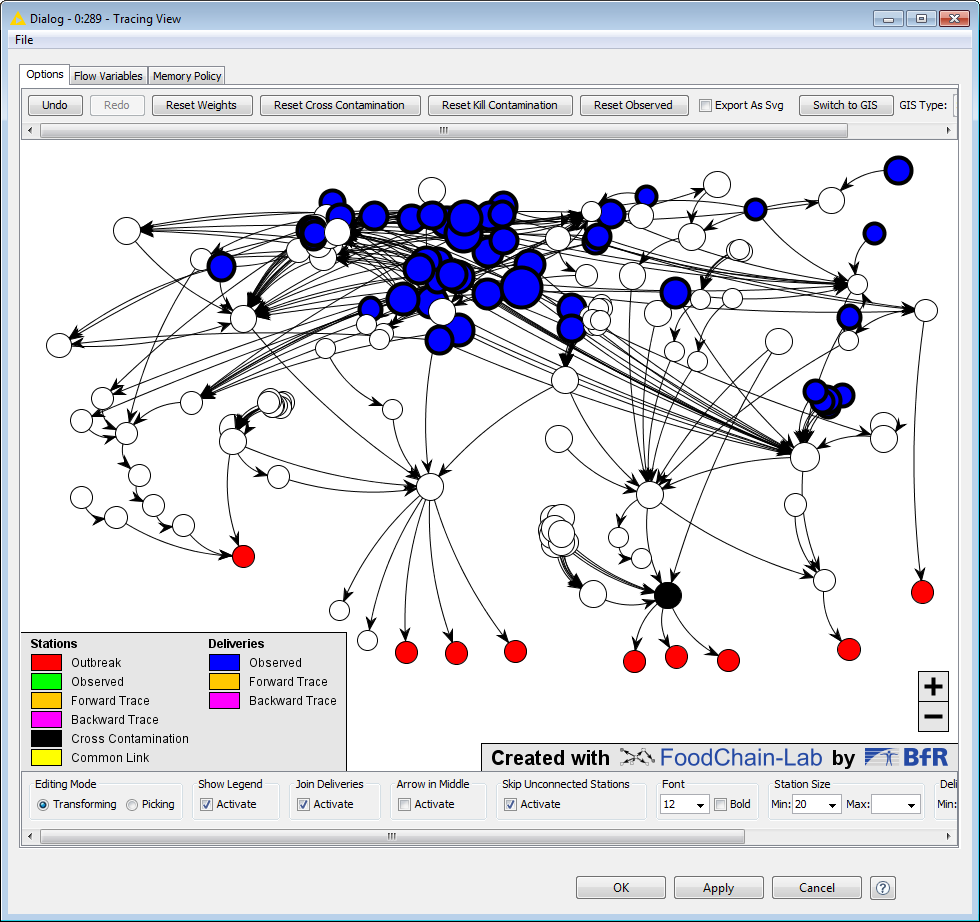
\includegraphics[height=0.6\textheight]{13.png}
	\end{center}
	\begin{itemize}
		\item All French primary producers have been clustered to cities.
		\item Each selected station (blue circle) is a French city.
	\end{itemize}
\end{frame}

\section{14}
\begin{frame}
	\begin{center}
  		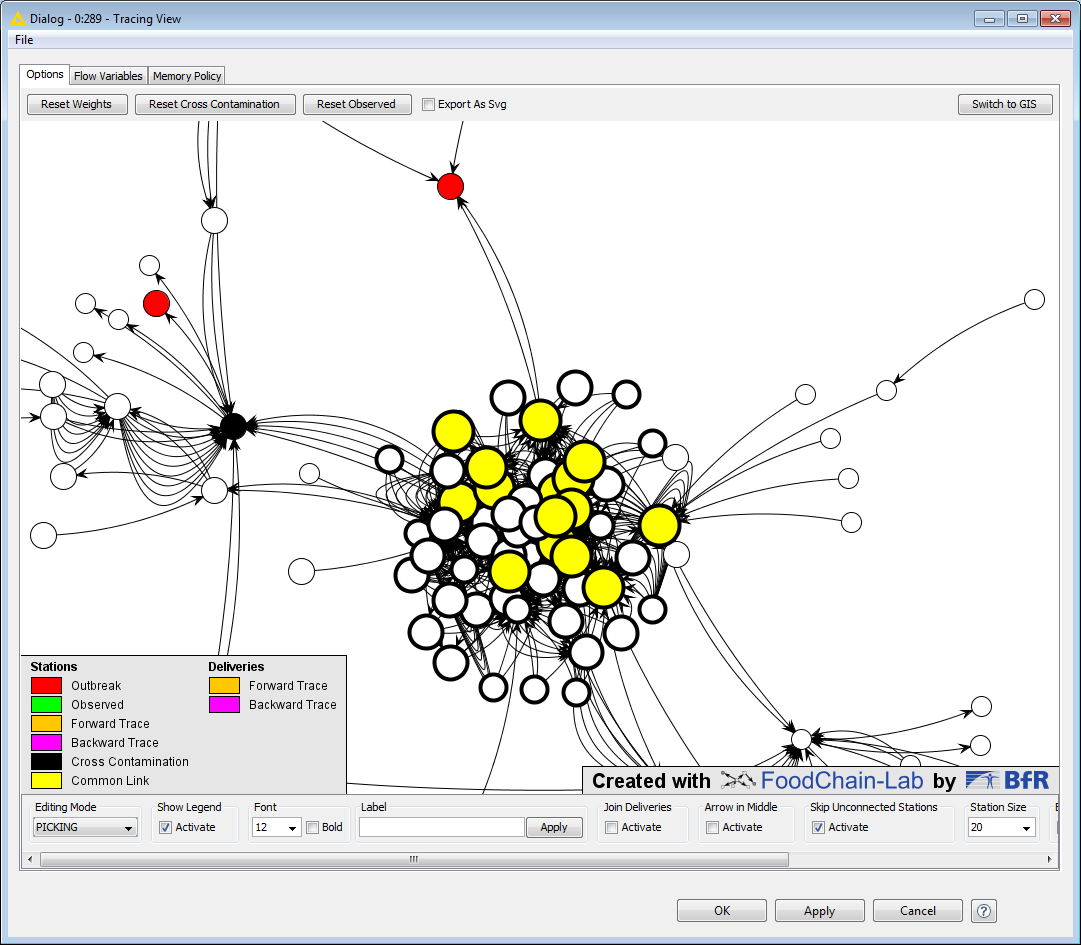
\includegraphics[height=0.6\textheight]{14.png}
	\end{center}
	\begin{itemize}
		\item Select "Picking" as \textbf{Editing Mode} and click in the graph to unselect all stations.
		\item You can now see, that one of the stations is yellow. That means, that this station (French city) is connected to all outbreak spots (red circles).
	\end{itemize}
\end{frame}

\section{15}
\begin{frame}
	\begin{center}
  		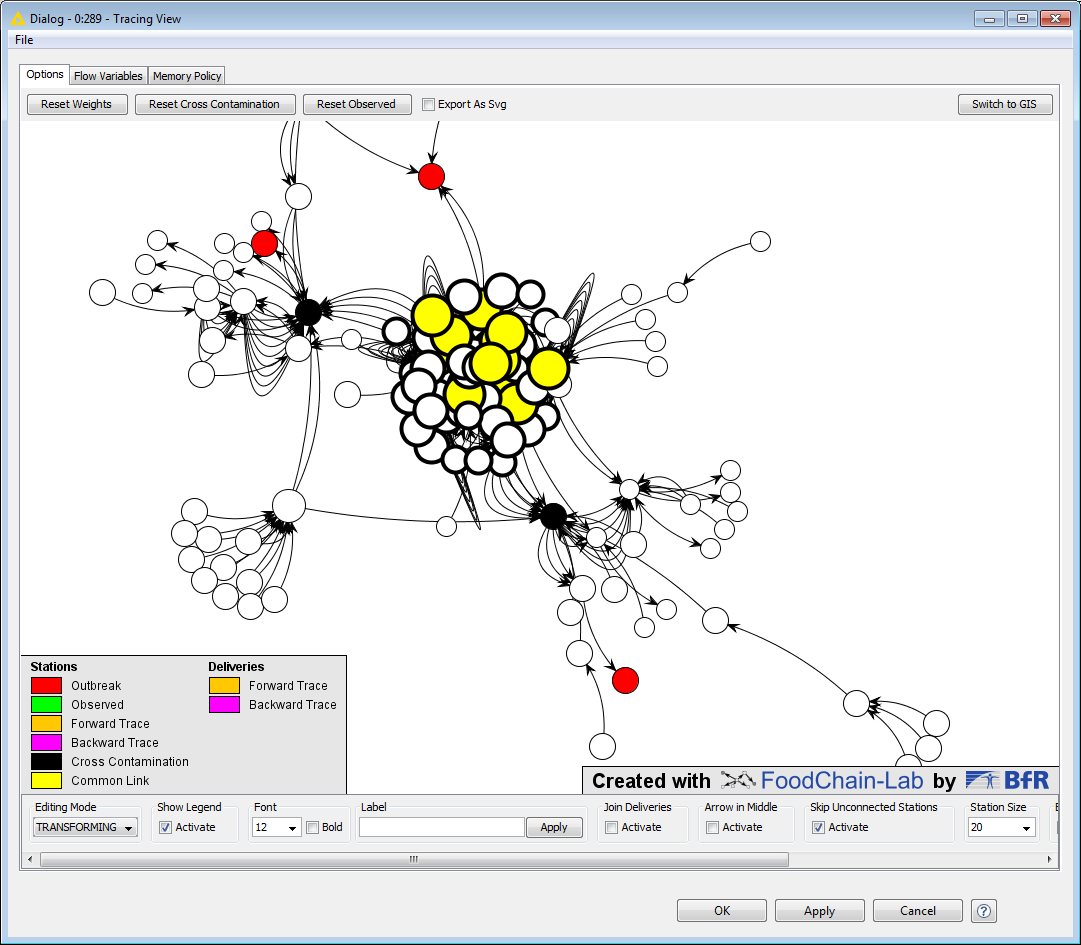
\includegraphics[height=0.6\textheight]{15.png}
	\end{center}
	\begin{itemize}
		\item Since the graph looks confusing now, we should reapply the layout algorithm.
		\item Right click in the graph and select \textbf{Apply Layout $>$ Fruchterman-Reingold} in the context menu.
	\end{itemize}
\end{frame}

\section{16}
\begin{frame}
	\begin{center}
  		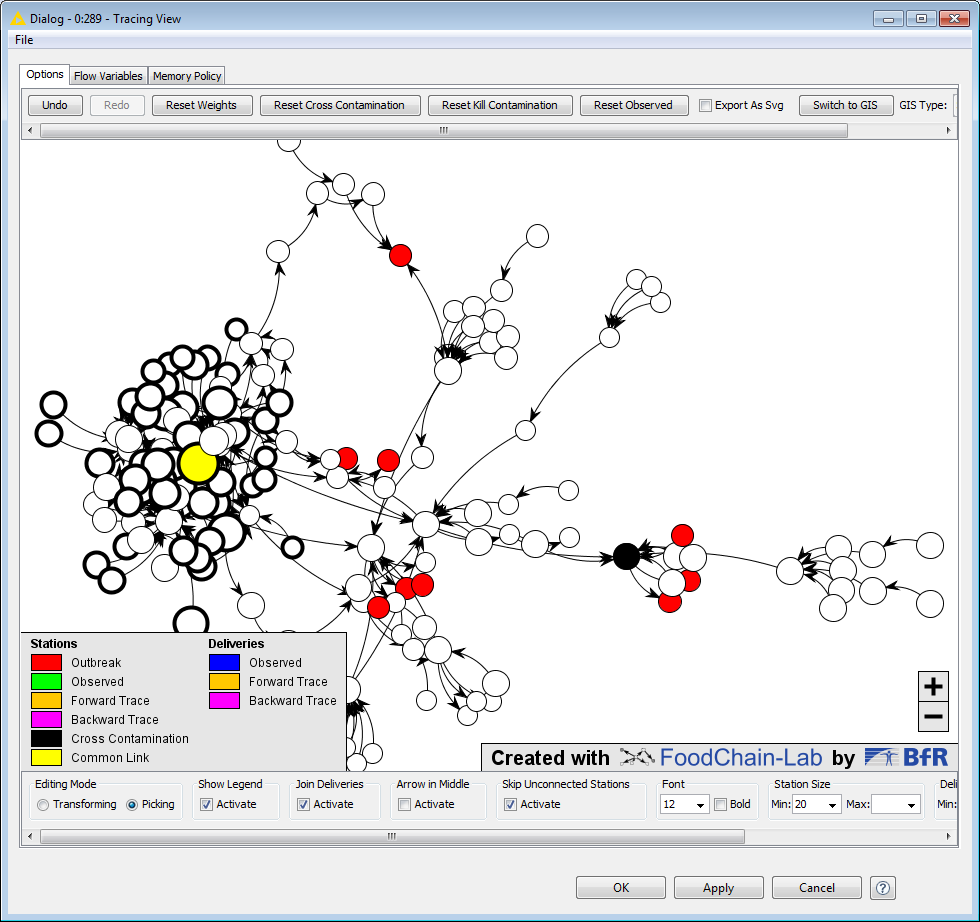
\includegraphics[height=0.6\textheight]{16.png}
	\end{center}
	\begin{itemize}
		\item The stations should be arranged in better way now.
		\item The algorithm is not deterministic, therefore your result will look different from the screenshot.
		\item To see which city is connected to all outbreak spots double click on the yellow circle.		
	\end{itemize}
\end{frame}

\section{17}
\begin{frame}
	\begin{center}
  		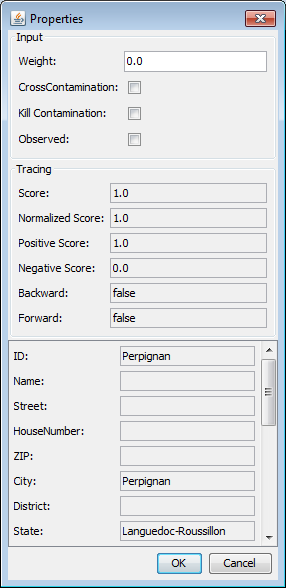
\includegraphics[height=0.6\textheight]{17.png}
	\end{center}
	\begin{itemize}
		\item As you can see in the dialog the city is "Perpignan".
	\end{itemize}
\end{frame}

\end{document}